We adjusted the CDB width to address a significant performance bottleneck observed when the width was set to 1. Specifically, with only one CDB available, the CDB stall rate reached approximately 45\%. This high stall rate caused functional units to be occupied longer and prevented completed instructions from writing their results back to the register file. As a result, dependent instructions could not be issued on time, stalling the pipeline and increasing overall CPI.
\begin{figure}[htbp]
  \centering
  \begin{minipage}[t]{0.24\textwidth}
    \centering
    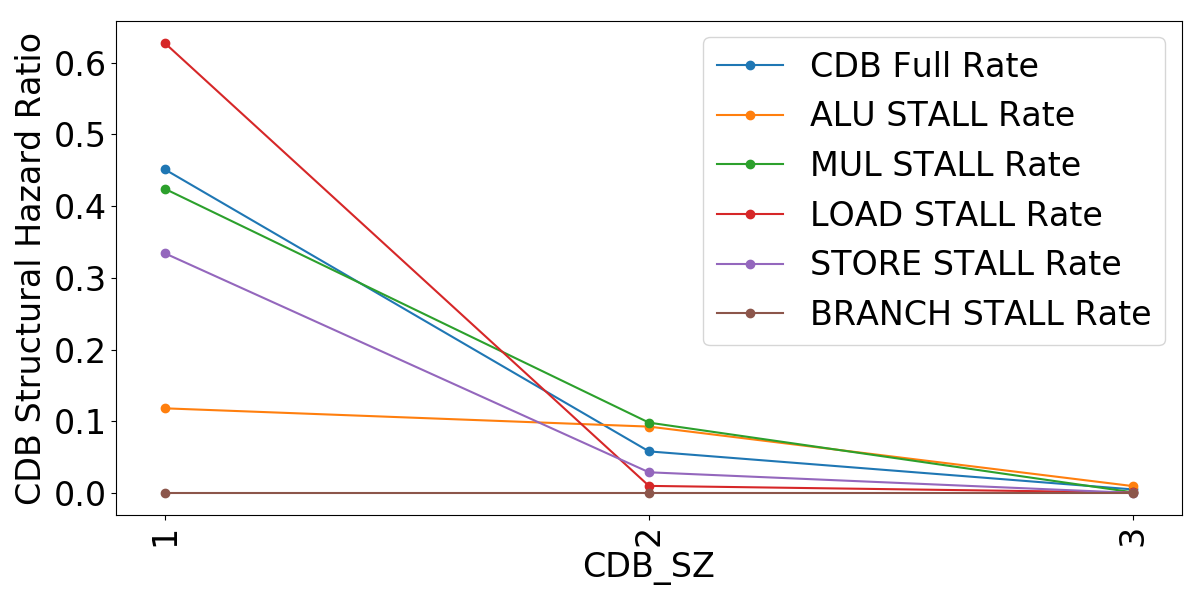
\includegraphics[width=\textwidth]{figures/Analysis/N-way/CDB_Stru.png}
    \caption{CDB Size vs. CDB Stall Rate}
    \label{fig:cdb_stall}
  \end{minipage}
  \hfill
  \begin{minipage}[t]{0.24\textwidth}
    \centering
    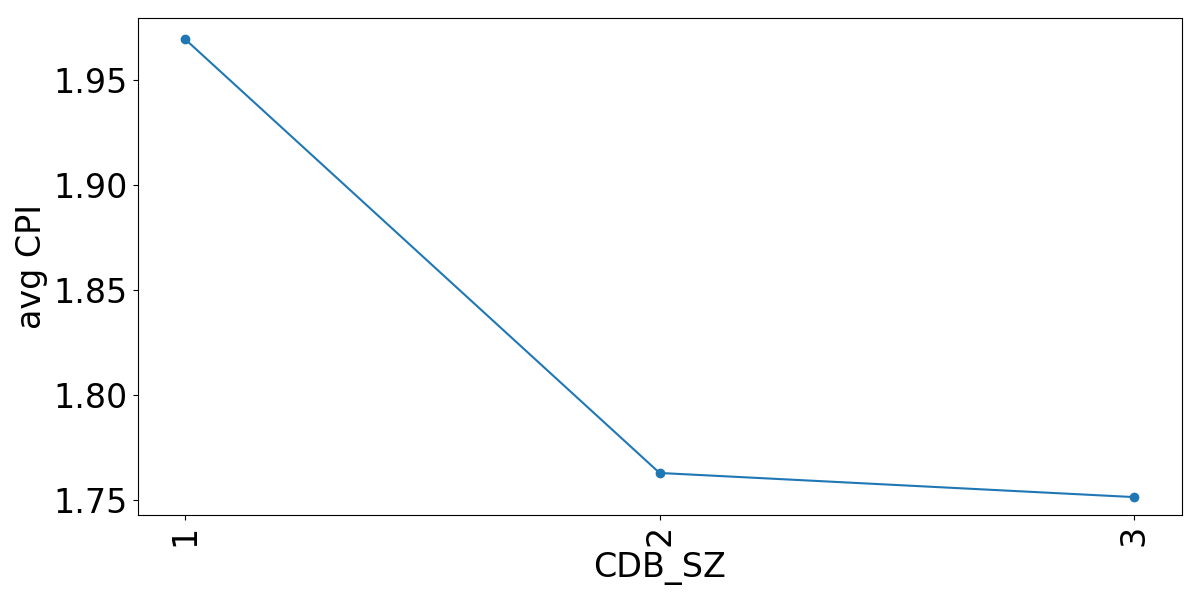
\includegraphics[width=\textwidth]{figures/Analysis/N-way/cpi_CDB.png}
    \caption{CDB Size vs. CPI}
    \label{fig:cdb_cpi}
  \end{minipage}
\end{figure}

The detailed result is shown in Figure~\ref{fig:cdb_stall}. We can see that the branch stall rate is always 0, and this is because we always prioritize branch instructions to resolve possible branch mispredictions earlier.

As shown in Figure~\ref{fig:cdb_stall}, each time the CDB width was increased by 1, the CDB stall rate dropped by approximately 8 times, and as shown in Figure~\ref{fig:cdb_cpi}, the CPI improved by roughly 10\%. These results demonstrate that increasing the CDB width effectively alleviates CDB bottlenecks, enabling faster instruction completion and reducing CPI.